\documentclass[xcolor=dvipsnames,hyperref={pdfpagelabels=false}]{beamer}

\usetheme{Boadilla}

\newcommand{\bi}{\begin{itemize}}
\newcommand{\ei}{\end{itemize}}
\newcommand{\be}{\begin{enumerate}}
\newcommand{\ee}{\end{enumerate}}
\newcommand{\bc}{\begin{center}}
\newcommand{\ec}{\end{center}}
\newcommand{\bd}{\begin{description}}
\newcommand{\ed}{\end{description}}
\newcommand{\I}{\item}
\newcommand{\f}{\frame}
\newcommand{\ft}{\frametitle}

\title{Offline Software Overview}
\subtitle{GlueX Collaboration Meeting}
\author[Mark Ito]{Mark M.\ Ito}
\date{February 22, 2013}
\institute[JLab]{Jefferson Lab}

\begin{document}

\f{\titlepage

}\f{\ft{Other Talks in This Session}

\bi\I Data Challenge: Richard Jones
\I CCDB: Dmitry Romanov
\I Tracking: Simon Taylor
\I Physics Analysis Tools: Paul Mattione
\ei

}\f{\ft{CCDB}

\bi
\I CCDB switched to Python code base: ccdb-shell, web page, command line tools
\I C++ code remains for read-operations, JANA jobs
\I Official version is now the database (new constants go into the CCDB)
\I Deployed in three places:
  \bi
  \I MySQL server at JLab, read/write, inside firewall
  \I MySQL server at JLab, read-only, open to world
  \I SQLite file, available from group disk at JLab
  \ei
\I Old text file system still works, deprecated, frozen
\I Caveat: intermittent ``hangs'' from MySQL server, possibly network related
\ei

}\f{\ft{Resources}
\bi
\I Large files, not well suited to relational database, like magnetic field maps
\I System for creating local cache
\I Resource entity could be controlled with CCDB
\I David developed this as part of the JANA framework
\I Goal: include in next release, migrate the magnetic fields maps
\ei

}\f{\ft{ROOT-based event display: EVE}
  \bi\I Dmitry did some exploratory work
  \I Used by LHC experiments
  \I Geometry based on HDDS, like simulation and reconstruction (we already have HDDS-to-ROOT convertor)
  \I Could be configured as JANA plug-in: full access to all raw and reconstructed objects
  \ei

}\f{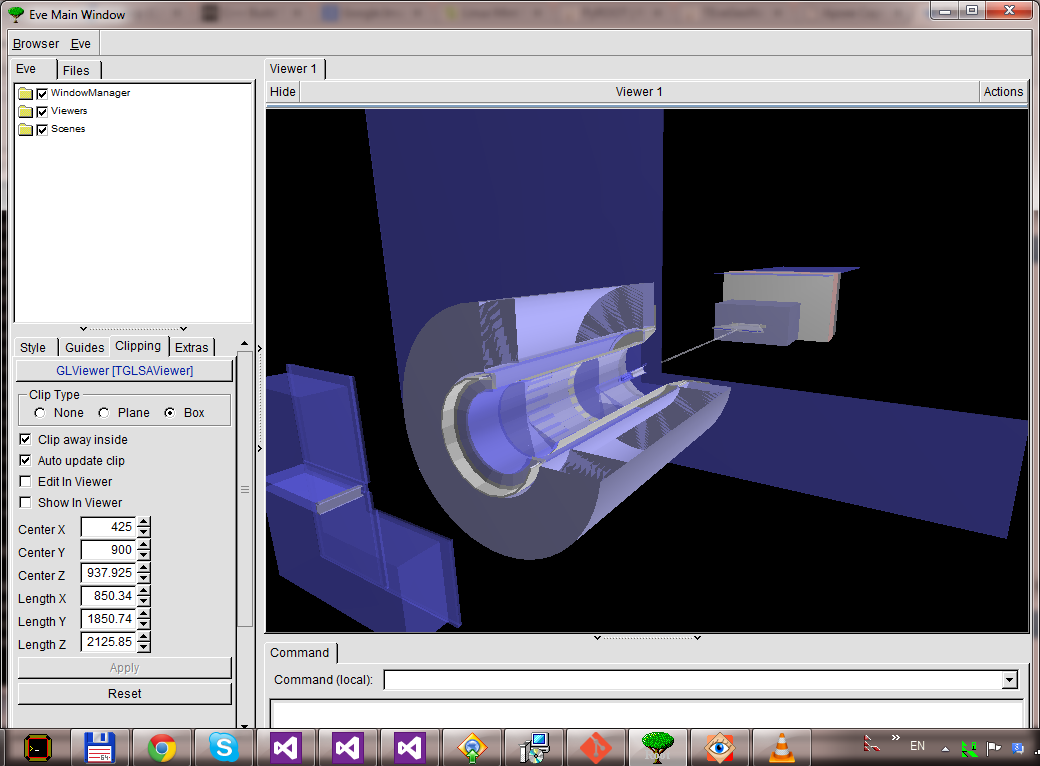
\includegraphics[width=\textwidth]{eve1.png}}
\f{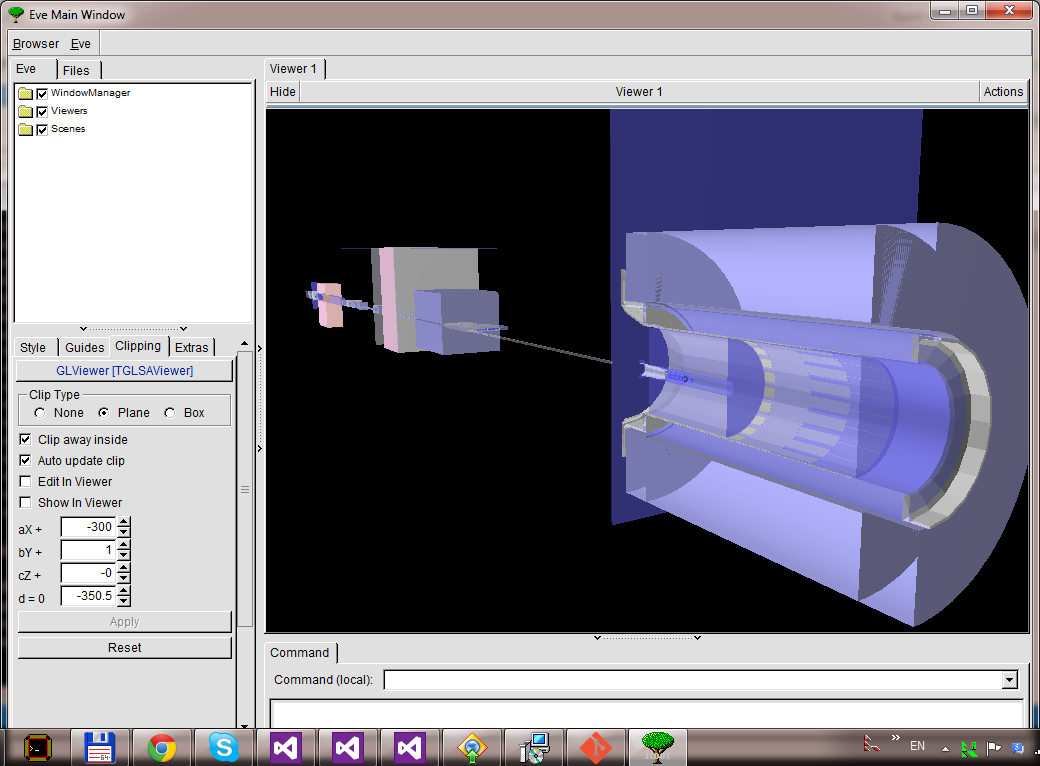
\includegraphics[width=\textwidth]{eve2.png}}
\f{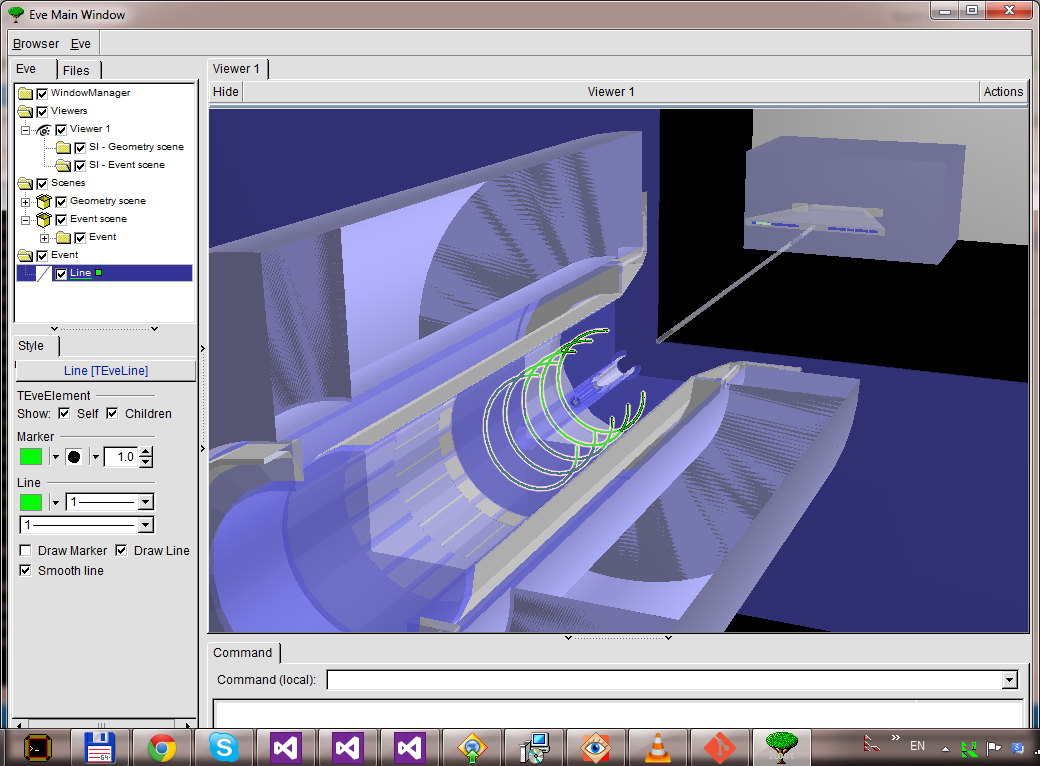
\includegraphics[width=\textwidth]{eve3.png}}
\f{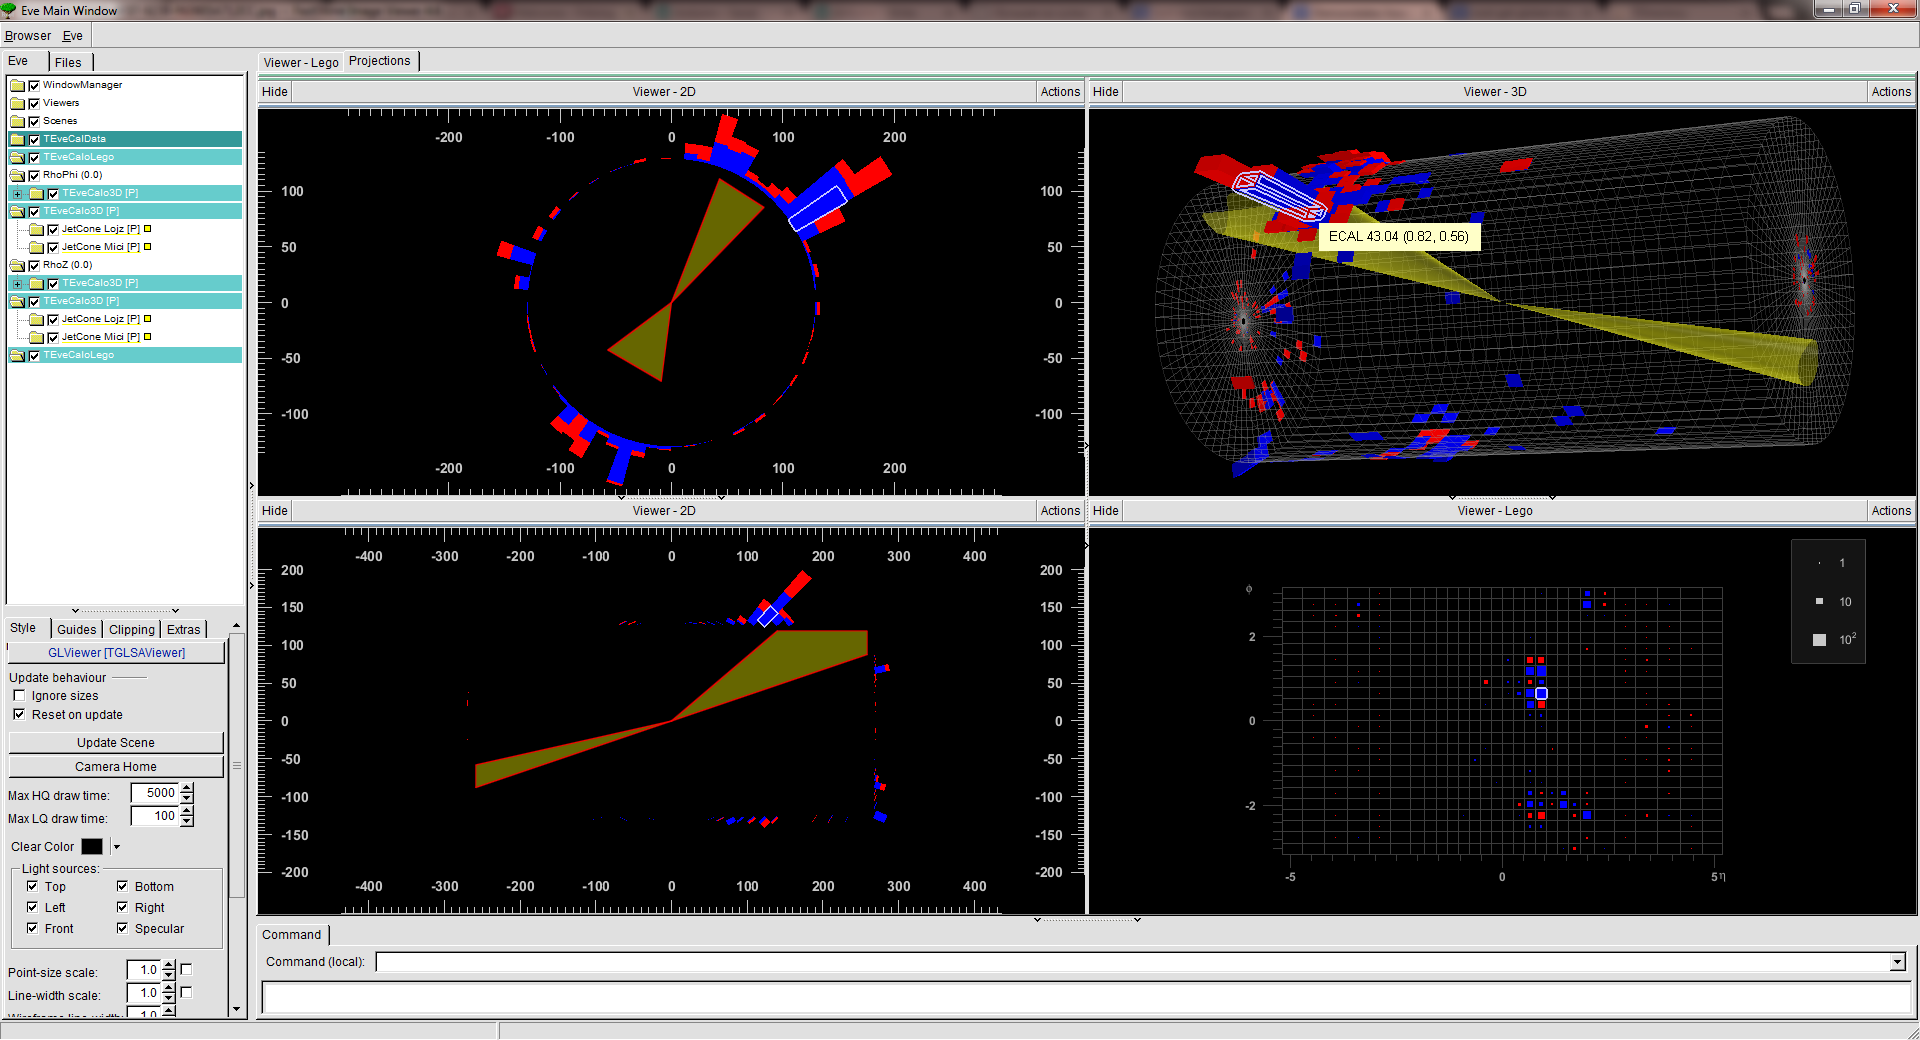
\includegraphics[width=\textwidth]{eve6.png}

}\f{\ft{Miscellanous}

\bi
\I Geometry Changes
  \bi
  \I Stereo/axial layer arrangement
  \I Overlaps of BCAL and FDC cables and FDC survey monuments
  \I Outer aluminum backing on BCAL added
  \I BCAL readout box masking some material
  \ei
\I Simulated raw data in EVIO format
\I Light-weight email lists: nightly builds, b1pi test, single-track test
\ei

}\f{\ft{Tasks}
\begin{columns}[t]
\column{0.33\textwidth}
\centerline{Simulation/Reconstruction}
\bi\small
\I photon clusters
  \bi
  \I hadronic contamination
  \I split of single showers
  \I merged photons
  \ei
\I conversion to Geant4
\I further tests of reconstruction code
\I event generator development
\I measurement error verification
\I event display
\ei
\column{0.33\textwidth}
\centerline{Software/Data}
\centerline{Management}
\bi
\I plan next data challenge
\I data distribution
\I micro-DST format
\I profiling code
\I unit testing
\I conversion to git
\I amplitude analysis code management
\I MySQL replication
\I project management
\ei
\column{0.33\textwidth}
\centerline{Documentation}
\bi
\I write the data challenge report
\I CCDB documentation
\I Doxygen configuration
\ei
\end{columns}

}

\end{document}
